\section{РЕАЛИЗАЦИЯ СТЕНДА}

\subsection{Разработка программного обеспечения для микроконтроллеров ESP32}

Для реализации учебного лабораторного стенда в качестве основной среды разработки была выбрана \textbf{Arduino IDE}. Это кроссплатформенное приложение с открытым исходным кодом, которое благодаря поддержке сторонних ядер позволяет программировать широкий спектр микроконтроллеров, включая семейство ESP32 от компании Espressif Systems.

\subsubsection{Среда разработки Arduino IDE и работа с ESP32}

Arduino IDE предоставляет удобный графический интерфейс для написания кода на языке C++ (с упрощенным синтаксисом), компиляции проектов и загрузки прошивок в микроконтроллеры через USB-интерфейс.

\begin{figure}[H]
\centering
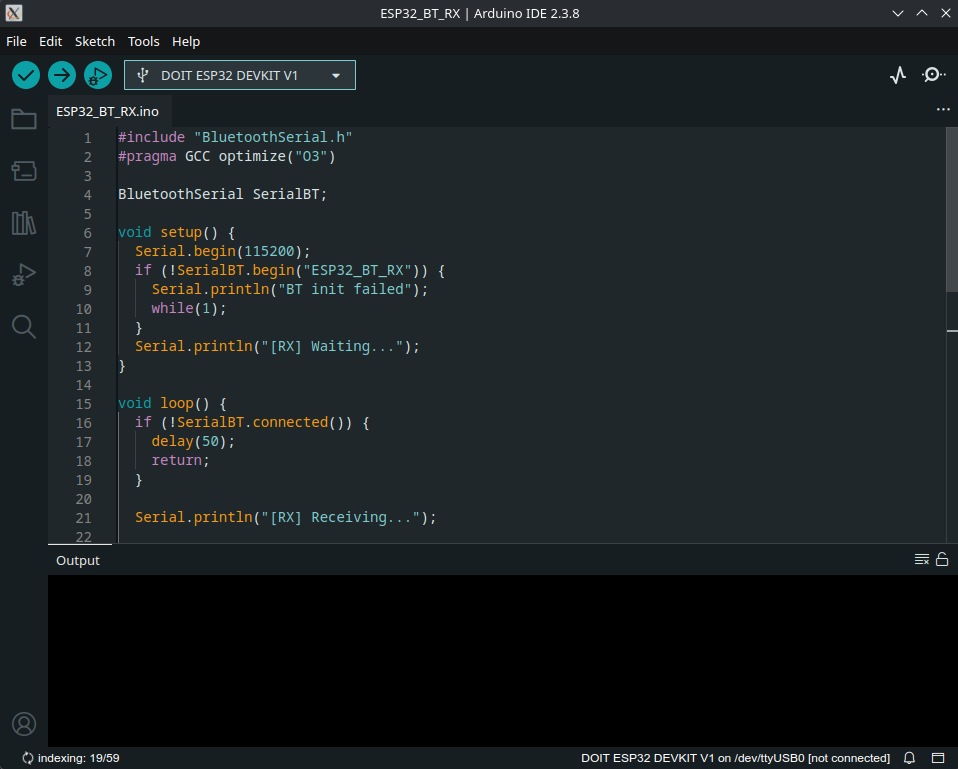
\includegraphics{figures/arduino_ide.png}
\caption{Интерфейс Arduino IDE}
\label{fig:arduino_ide}
\end{figure}

Процесс настройки ~\cite{esp32_arduino_configuration} и работы с ESP32 в данной среде включает следующие этапы:
\begin{enumerate}[nosep]
    \item \textbf{Установка поддержки плат ESP32:} В настройках Arduino IDE (\textit{File $\rightarrow$ Preferences}) в поле \textit{Additional Boards Manager URLs} добавляется ссылка на репозиторий Espressif: \texttt{https://raw.githubusercontent.com/espressif/arduino-esp32/gh-pages/package\_esp32\_index.json}. После этого через \textit{Tools $\rightarrow$ Board $\rightarrow$ Boards Manager} устанавливается пакет \textit{esp32 by Espressif Systems}.
    \item \textbf{Выбор конфигурации платы:} В меню \textit{Tools} выбирается конкретная модель модуля (например, \textit{ESP32 Dev Module}), частота процессора, размер флеш-памяти и скорость загрузки.
    \item \textbf{Настройка порта:} Выбирается соответствующий последовательный порт (\texttt{/dev/ttyUSB0} или \texttt{/dev/ttyACM0} в Linux), через который осуществляется связь с микроконтроллером.
    \item \textbf{Компиляция и загрузка:} Код компилируется в машинный код для архитектуры Xtensa LX6/LX7 и загружается в память ESP32. При загрузке микроконтроллер автоматически переходит в режим программирования благодаря схеме автопереключения сигналов DTR/RTS.
\end{enumerate}

Такой подход позволяет студентам сосредоточиться на логике работы протоколов Bluetooth, абстрагируясь от низкоуровневой настройки регистров контроллера, что соответствует целям дисциплины «Сети связи».

\subsubsection{Библиотеки для работы с Bluetooth в ESP32}

Ядро ESP32 для Arduino предоставляет множество библиотек для работы с беспроводными интерфейсами ~\cite{esp32_arduino_github}. Вот некоторые из них, которые были использованы при разработке лабораторного стенда.

\paragraph{1. Библиотека \texttt{BluetoothSerial.h} (Classic Bluetooth)}
Данная библиотека реализует профиль SPP (Serial Port Profile) поверх стека классического Bluetooth (BR/EDR). Она эмулирует последовательный порт UART, позволяя передавать данные между устройствами так же просто, как при использовании проводного соединения.

\textbf{Основной функционал:}
\begin{itemize}[nosep]
    \item \texttt{begin(name, isMaster)}: Инициализация Bluetooth-модуля. Параметр \texttt{name} задает видимое имя устройства, а \texttt{isMaster} определяет роль (ведущий или ведомый).
    \item \texttt{connect(address)}: Метод для инициирования подключения к удаленному устройству по его MAC-адресу (для режима Master).
    \item \texttt{available()}, \texttt{read()}, \texttt{write()}: Стандартные методы потокового ввода-вывода, аналогичные работе с объектом \texttt{Serial}. Они обеспечивают буферизацию данных и управление потоком.
    \item \texttt{connected()}: Проверка статуса активного соединения.
\end{itemize}

Эта библиотека идеально подходит для задач передачи больших объемов данных с высокой скоростью, таких как измерение пропускной способности канала в режиме EDR.

\paragraph{2. Библиотека \texttt{BLEDevice.h} (Bluetooth Low Energy)}
Для работы с BLE используется более сложный набор классов, предоставляющих доступ к протоколам GAP (Generic Access Profile) и GATT (Generic Attribute Profile). Эта библиотека не эмулирует последовательный порт, а оперирует понятиями сервисов, характеристик и дескрипторов.

\textbf{Ключевые классы и их функционал:}
\begin{itemize}[nosep]
    \item \textbf{\texttt{BLEDevice}}: Управляет глобальной инициализацией стека BLE, сканированием эфира и созданием клиентов/серверов.
    \item \textbf{\texttt{BLEServer} / \texttt{BLEClient}}: Реализуют логику периферийного устройства (Peripheral) или центрального устройства (Central). Сервер создает сервисы, клиент подключается к ним.
    \item \textbf{\texttt{BLEService}}: Представляет собой контейнер для характеристик, идентифицируемый уникальным UUID.
    \item \textbf{\texttt{BLECharacteristic}}: Основной элемент хранения данных. Позволяет задавать свойства доступа (\texttt{PROPERTY\_READ}, \texttt{PROPERTY\_WRITE}, \texttt{PROPERTY\_NOTIFY}). Поддерживает механизм обратных вызовов (callbacks) для обработки событий записи или чтения.
    \item \textbf{\texttt{BLE2902}}: Специальный класс для создания дескриптора CCCD (Client Characteristic Configuration Descriptor), необходимого для включения уведомлений (Notifications) и индикаций (Indications).
    \item \textbf{\texttt{setMTU(size)}}: Метод для согласования максимального размера блока передачи (MTU) между центральным и периферийным устройствами, что критически важно для оптимизации скорости передачи в BLE.
\end{itemize}

Использование этих библиотек позволяет гибко конфигурировать параметры соединения, такие как интервал рекламы, мощность передатчика и размеры пакетов, что необходимо для выполнения сравнительного анализа скоростных характеристик различных режимов работы Bluetooth.

\subsection{Анализ трафика Bluetooth с использованием Wireshark}

Для глубокого понимания работы протоколов Bluetooth стенд поддерживает детальный анализ сетевого трафика с использованием профессионального анализатора протоколов \textbf{Wireshark}. Данный инструмент позволяет визуализировать обмен данными на всех уровнях стека Bluetooth, от физического до прикладного.

\subsubsection{Принцип перехвата пакетов в Wireshark}

Wireshark не является самостоятельным драйвером захвата для Bluetooth в Linux. Он работает как интерфейс отображения и декодирования, получая данные от низкоуровневых утилит ядра. Принцип перехвата строится на использовании интерфейса \textbf{HCI (Host Controller Interface)}.

Существует два основных способа организации потока данных для Wireshark:

\begin{enumerate}[nosep]
    \item \textbf{Захват через сокет HCI (Linux Bluetooth Socket):}
    Wireshark обращается к системному сокету \texttt{bluetooth0} (или аналогичному), который предоставляет ядро Linux. В этом режиме Wireshark перехватывает пакеты, проходящие между операционной системой (Host) и Bluetooth-контроллером.

    \item \textbf{Захват через утилиту btmon (BTSnoop формат):}
    Утилита \texttt{btmon}, входящая в пакет BlueZ, перехватывает сырые HCI-команды и события и сохраняет их в формате \texttt{btsnoop} (стандартный формат для анализа Bluetooth). Wireshark нативно поддерживает этот формат.
\end{enumerate}

\subsubsection{Настройка среды для анализа}

Для корректной работы Wireshark с Bluetooth-трафиком необходимо выполнить ряд настроек в операционной системе Linux ~\cite{wireshark_setup}.

\paragraph{1. Предоставление прав пользователю}
По умолчанию захват сетевых пакетов требует прав суперпользователя (\texttt{root}). Для безопасной работы рекомендуется добавить текущего пользователя в группу \texttt{wireshark}.

Команда для добавления пользователя в группу:
\begin{lstlisting}[language=bash]
sudo usermod -a -G wireshark $USER
\end{lstlisting}
\textit{Примечание:} После выполнения команды необходимо перелогиниться в систему для применения изменений.

\paragraph{2. Установка необходимых компонентов}
Убедитесь, что установлены следующие пакеты:
\begin{lstlisting}[language=bash]
sudo apt install wireshark bluez-tools
\end{lstlisting}

\paragraph{3. Выбор интерфейса в Wireshark}
При запуске Wireshark в списке доступных интерфейсов необходимо выбрать \texttt{bluetooth0} (или другой с bluetooth в названии).

\begin{figure}[H]
\centering
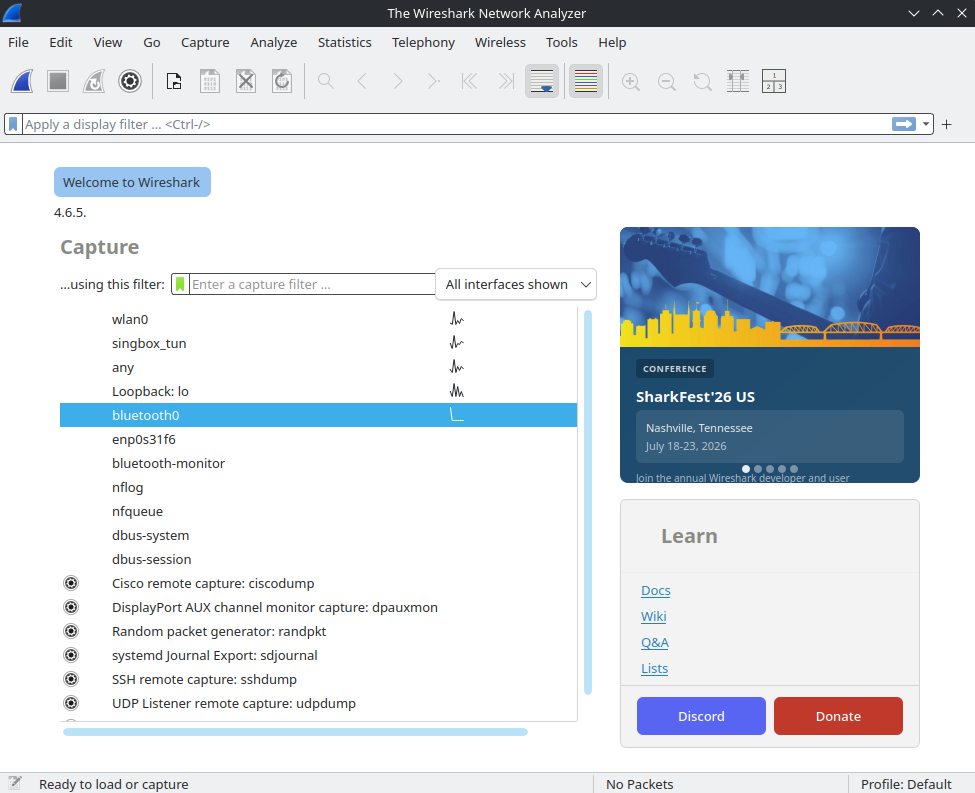
\includegraphics{figures/wireshark_main.png}
\caption{Меню выбора интерфейса}
\label{fig:wireshark_main}
\end{figure}

\subsubsection{Методика запуска анализа}

Работа с анализатором трафика в Wireshark осуществляется интуитивно понятно через графический интерфейс и состоит из следующих этапов:

\begin{enumerate}[nosep]
    \item \textbf{Выбор интерфейса и начало захвата:}
    В главном окне программы отображается список доступных сетевых интерфейсов. Для анализа Bluetooth-трафика необходимо выбрать интерфейс, соответствующий Bluetooth-адаптеру (обычно обозначается как \texttt{bluetooth0}, \texttt{hci0} или просто \texttt{Bluetooth}). Захват трафика начинается автоматически сразу после двойного клика по названию интерфейса или нажатия кнопки \textit{Start}.
    
    \item \textbf{Генерация трафика:}
    После начала записи следует выполнить целевые действия с Bluetooth-устройствами (например, сопряжение, подключение, передача данных), чтобы сформировать необходимый для анализа поток пакетов.
    
    \item \textbf{Остановка и сохранение:}
    По завершении действий запись останавливается нажатием красной кнопки \textit{Stop} на панели инструментов. Полученные данные можно сохранить в файл формата \texttt{pcapng} через меню \textit{File $\rightarrow$ Save As} для последующего изучения или включения в отчет.
    
    \item \textbf{Анализ и фильтрация:}
    В сохраненном или активном сеансе используется поле фильтра (в верхней части окна) для выделения конкретных протоколов или событий. Например, ввод \texttt{bthci} отобразит все служебные пакеты контроллера, а \texttt{btrfcomm} — данные профиля RFCOMM.
    
    \item \textbf{Формирование вырезок для отчета:}
    Для включения результатов в отчет выбирается интересующий пакет в списке, после чего делается скриншот нижней панели декодирования, где раскрыта структура выбранного протокола. Это позволяет наглядно продемонстрировать поля заголовков и содержимое полезной нагрузки.
\end{enumerate}

\subsubsection{Фильтрация и интерпретация данных}

Wireshark автоматически декодирует структуру пакетов Bluetooth. В панели деталей пакета (Packet Details) отображается иерархия:
\begin{enumerate}[nosep]
    \item \textbf{Bluetooth HCI H4/H5} — служебные заголовки шины HCI;
    \item \textbf{Bluetooth HCI Event/Command} — тип события (например, Inquiry Complete);
    \item \textbf{L2CAP} — заголовки логического канала;
    \item \textbf{RFCOMM / SDP / ATT / GATT} — протоколы верхнего уровня.
\end{enumerate}

Для удобства анализа используются дисплейные фильтры. В поле фильтра (Filter) вводятся следующие выражения:

\begin{table}[H]
\centering
\caption{Основные фильтры Wireshark для Bluetooth}
\label{tab:wireshark_filters}
\renewcommand{\arraystretch}{1.3}
\begin{tabularx}{\textwidth}{|X|X|}
\hline
\textbf{Фильтр} & \textbf{Описание} \\
\hline
bthci & Отображает все HCI-пакеты (база для любого анализа). \\
\hline
bthci\_cmd & Только HCI-команды (от Host к Controller). \\
\hline
bthci\_evt & Только HCI-события (от Controller к Host). \\
\hline
btl2cap & Пакеты протокола L2CAP. \\
\hline
btrfcomm & Трафик профиля RFCOMM (Classic Bluetooth). \\
\hline
btatt & Протокол ATT (основа BLE). \\
\hline
btgatt & Профиль GATT (структура сервисов BLE). \\
\hline
bthci\_evt.code == 0x03 & Событие завершения подключения (Connection Complete). \\
\hline
bthci\_evt.code == 0x2f & Расширенные результаты поиска (Extended Inquiry Result). \\
\hline
\end{tabularx}
\end{table}

Использование Wireshark позволяет студентам наглядно увидеть разницу между «сырым» эфирным обменом и логической структурой данных, обрабатываемой операционной системой, что критически важно для отладки прошивок и понимания работы стека протоколов.

\subsection{Конфигурация программного обеспечения стенда}

Для полноценной работы стенда требуется следующая конфигурация ПО:

\textbf{На стороне ПК:}
\begin{itemize}
    \item ОС Linux (Ubuntu 20.04+ или аналогичная) с ядром 5.0+;
    \item BlueZ 5.50+ (официальный стек Bluetooth для Linux);
    \item Wireshark 3.0+ с поддержкой Bluetooth;
    \item Python 3.8+ с библиотеками \texttt{pybluez}, \texttt{pyserial};
    \item Arduino IDE 1.8+ или PlatformIO для компиляции прошивок.
\end{itemize}

\textbf{На стороне ESP32:}
\begin{itemize}
    \item ESP-IDF (Espressif IoT Development Framework) или Arduino Core for ESP32;
    \item Библиотеки \texttt{BluetoothSerial.h} для Classic Bluetooth;
    \item Библиотеки \texttt{BLEDevice.h} для BLE.
\end{itemize}

\textbf{Дополнительные утилиты:}
\begin{itemize}
    \item \texttt{bluetoothctl} — интерактивный клиент для управления Bluetooth;
    \item \texttt{rfcomm} — привязка RFCOMM-устройств к tty;
    \item \texttt{hciconfig}/\texttt{hcitool} (устаревшие, но полезные для диагностики).
\end{itemize}
